\chapter{Система поиска пропавших домашних животных}
\label{ch:petsearch}

Система поиска пропавших домашних животных, реализованная в рамках проекта компании ООО "НКБТех"\ и в процессе выполнения данной бакалаврской работы, ставит свой целью отслеживание их передвижений в областях видимости различных городских камер видеонаблюдения. Для этого используется пайплайн из нескольких технологий компьютерного зрения и анализа данных, схема которого представлена на \hyperref[fig:petsearch_scheme]{Рисунке \ref*{fig:petsearch_scheme}}:

\begin{figure}[ht]
	\centering
	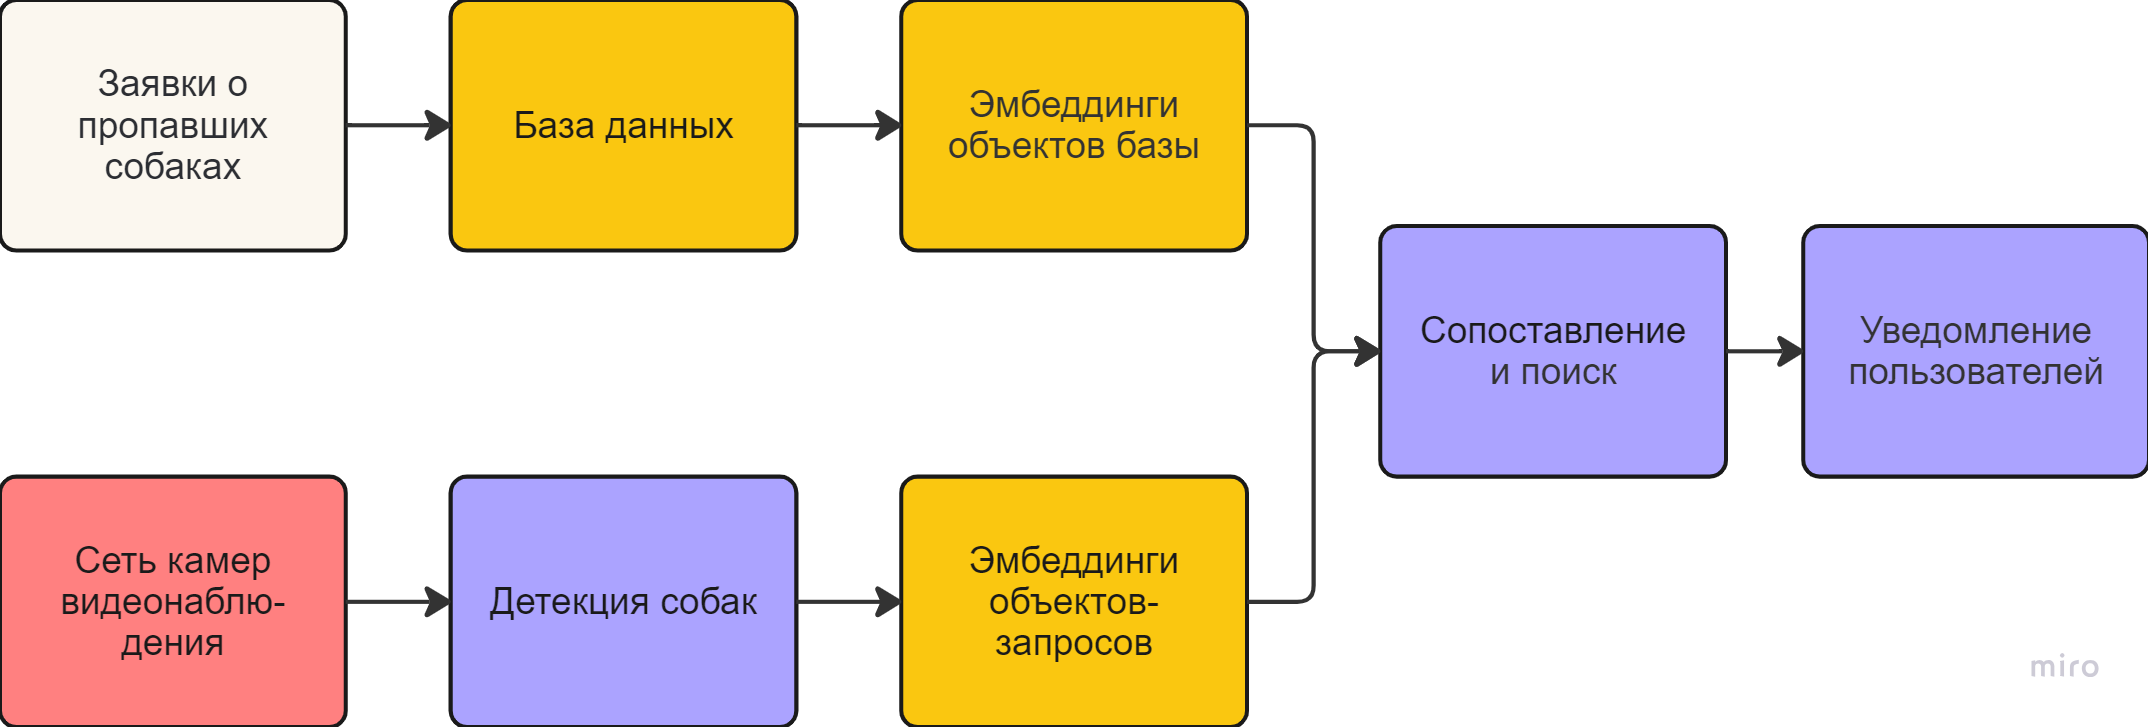
\includegraphics[width=0.9\textwidth]{images/petsearch/scheme.png}
	\caption{Схема работы системы поиска}
	\label{fig:petsearch_scheme}
\end{figure}

\begin{enumerate}
    \item Создание базы данных разыскиваемых животных

    \item Подключение городской системы видеонаблюдения к базе данных

    \item Детекция животных на видео

    \item Идентификация обнаруженного объекта с помощью техник Re-Id

    \item Поиск соответствий в базе данных

    \item Построение траектории движения в реальном времени

\end{enumerate}

На первом этапе формируется база данных из потерявшихся животных. В нее заносятся записи от пользователей, содержащие одну или несколько фотографий их питомца. Кроме этого, может быть предоставлена дополнительная информация в виде текстового описания, а также классификация по некоторым важным категориям. На текущем этапе развития проекта в качестве питомцев рассматриваются только собаки, соответственно, признаки классификации выбраны специфичными именно для них. Согласно Российской кинологической федерации, наиболее информативными признаками для описания собак являются цвет, размер, длина лап относительно туловища, длина морды, форма ушей и тип шерсти. В дальнейшем поиск производится на основе всей имеющейся информации.

Далее выполняется подключение к камерам городского видеонаблюдения. Суммарно на данном этапе реализации проекта доступно несколько сотен камер в пределах одного района. 

Затем сервис обработки видеопотока подает кадры с камер в модель компьютерного зрения для детекции объектов. Среди результатов детекции отбираются те, которые соответствуют классу "собака".

После этого каждый обнаруженный \bbox, содержащий собаку, с помощью Re-Id модели переводится в эмбеддинг, который затем сравнивается с эмбеддингами изображений из базы данных. Также с помощью отдельной модели может быть произведена классификация для фильтрации по соответствию основных признаков. Также с помощью мультимодальных моделей, таких как CLIP \cite{radford2021learning} и CLIP-ReID \cite{li2023clip} может быть построено соответствие текстовому описанию. Исходя из метрической близости эмбеддингов находятся соответствия с объектами базы. Таким образом, отбирается одна или несколько записей, которые соответствуют обнаруженной в данной момент собаке, и соответствующим пользователям присылаются уведомления об обнаружении животного.

Наконец, поскольку обработка видеопотока, детекция и поиск происходят в режиме реального времени, возможно построение траектории движения обнаруженной собаки между областями обзора камер, следуя которой можно достичь местоположения животного.


\section{Датасеты}

Существует несколько публичных датасетов, посвященных методам обработки изображений животных. Основные датасеты, сфокусированные на изображениях собак $-$ Tsinghua Dog \cite{Zou2020ThuDogs} и Stanford Dog \cite{khosla2011novel}. Они содержат разметку на породы собак, включающую в себя большое количество категорий и подкатегорий.

Однако с точки зрения системы поиска классификация по породам не всегда является оптимальной. Так, собаки одной и той же породы могут иметь разный цвет, или же разные комбинации цветов, и в таком случае именно дифференциация по цвету будет являться более информативной. Также собаки некоторых пород, например, пуделей, встречаются как больших размеров, так и карликовые.

В связи с этим в рамках разработки проекта компанией был собран собственный датасет классификации собак. Он включает в себя $50\ 000$ изображений собак с выставки и разметку для 6 категорий. Пример изображений из датасета можно увидеть на \hyperref[fig:petsearch_dataset]{Рисунке \ref*{fig:petsearch_dataset}}. Изображения собак представляют собой фотографии с выставки, обработанные с помощью выделения \bbox-ов, содержащих собак, благодаря чему наблюдается высокая репрезентативность как по породам, так и по классификационным признакам. В \hyperref[tab:datasets_dog]{Таблице \ref*{tab:datasets_dog}} приведены описания признаков классификации.

\begin{figure}[ht]
	\centering
	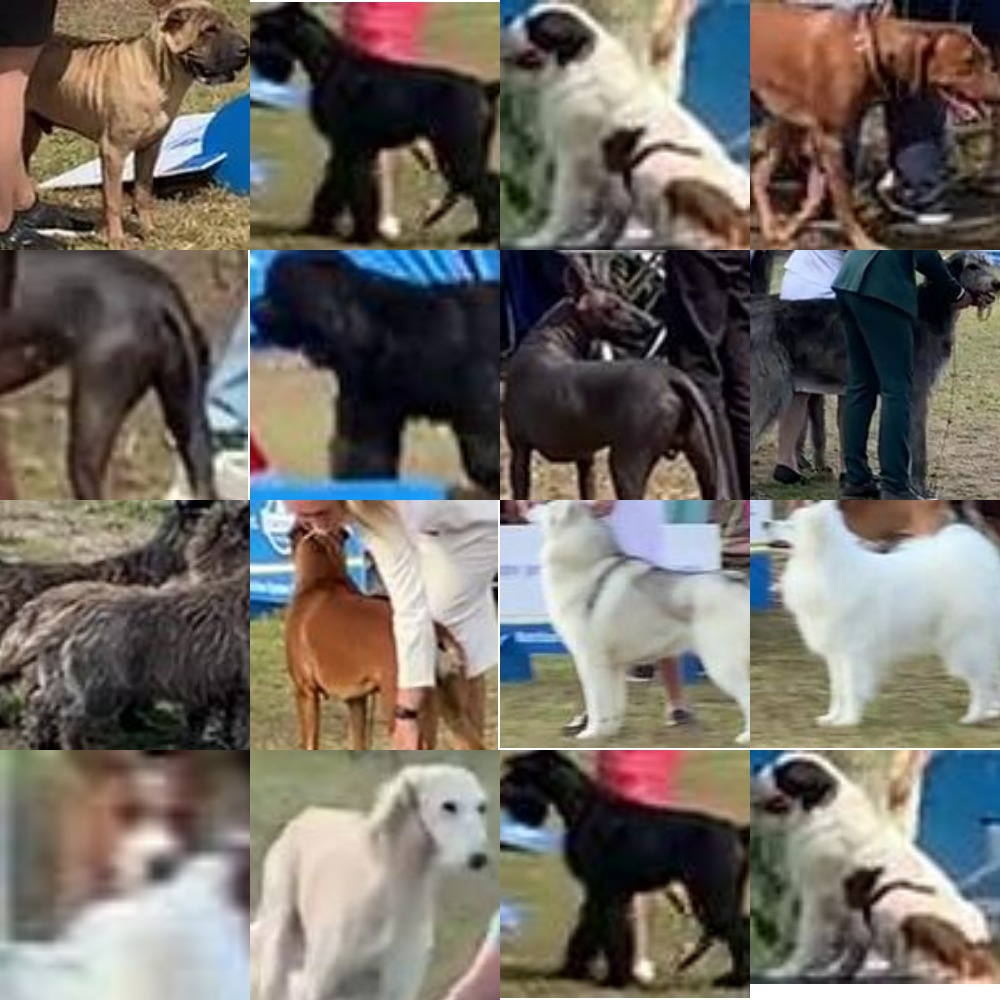
\includegraphics[width=0.7\textwidth]{images/petsearch/dataset.jpg}
	\caption{Пример изображений из датасета}
	\label{fig:petsearch_dataset}
\end{figure}

\begin{table}[]
    \centering
    \caption{Категории классификации в датасете}
    \begin{tabular}{|l|l|l|}
        \hline
        \multicolumn{1}{|l|}{Признак} & \multicolumn{1}{l|}{Количество значений} & 
        \multicolumn{1}{l|}{Значения}\\ \hline
        Цвет & 11 & белый, бежевый, \\ & & черно-белый, черно-рыже-белый, \\ & & черно-рыжий, черно-серый, \\ & & черный, серый, \\ & & рыжий, коричневый, \\ & & коричнево-белый \\ \hline
        Размер & 3 & большой, средний, малый \\ \hline
        Длина лап & 2 & длинные, короткие \\ \hline
        Тип ушей & 3 & стоячие, полу-висячие, \\ & & стоячие \\ \hline
        Тип морды & 2 & длинная, короткая \\ \hline
        Тип шерсти & 5 & длинношерстный, среднешерстный, \\ & & гладкошерстный, безшерстный, \\ & & курчавый \\ \hline
    \end{tabular}
    \label{tab:datasets_dog}
\end{table}

К сожалению, ни один из датасетов не предоставляет разметки напрямую для задачи Re-Id. Таким образом, измерить качество решения данной задачи можно лишь косвенно, то есть на основе вспомогательной информации, опираясь на качество решения задачи классификации или с помощью визуальной оценки ранжированных списков.


\section{Решение с помощью классификации}

Таким образом, в данной постановке возможно решить задачу классификации объектов. Для классификации собак по породам существуют решения, имеющие качество, близкое к $100 \%$ \cite{bera2022sr}. Однако классификация по специфичным признакам, представленным в нашем датасете, является более сложной задачей и на данный момент не имеет решения с высоким качеством.

В рамках исследования были проведены эксперименты по обучения ML-моделей для классификации собак. Процесс обучения строился в двух вариантах: в первом варианте для каждого признака обучалась своя модель, а во втором обучалась одна модель с шестью классификаторами на выходе. Оба способа показали схожее качество. Репозиторий с кодом, использованным для проведения экспериментов, доступен по ссылке: \href{https://github.com/nkb-tech/nkb-classification}{https://github.com/nkb-tech/nkb-classification}.

Были проверены различные архитектуры моделей: ResNet \cite{he2015deep}, MobileNet \cite{howard2017mobilenets}, EfficientNet \cite{tan2019efficientnet}, ViT \cite{dosovitskiy2020image}, ConvNext \cite{liu2022convnet}. Также были сравнены различные методы оптимизации: Adam \cite{kingma2017adam}, AdamW \cite{loshchilov2019decoupled}, RAdam \cite{liu2021variance}, NAdam \cite{dozat2016incorporating}. Кроме этого были проверены функции потерь Cross-Entropy и FocalLoss \cite{lin2017focal}. Также применялись различные аугментации данных, связанные с добавлением шума, размытости, изменением цвета, закрытия части кадра. Наилучший результат показало сочетание ConvNext-Base + RAdam + Cross-Entropy.


Были измерены две метрики многоклассовой классификации: Balanced accuracy и ROC AUC, представляющие собой соответственно усредненные по всем классам значения recall и ROC AUC. Результаты экспериментов приведены в \hyperref[tab:classification_results]{Таблице \ref*{tab:classification_results}}.

\begin{table}[]
    \centering
    \caption{Качество классификации собак по 6 признакам}
    \begin{tabular}{|l|l|l|}
        \hline
        \multicolumn{1}{|l|}{Признак} & \multicolumn{1}{l|}{Balanced Accuracy, \%} & 
        \multicolumn{1}{l|}{ROC AUC, \%}\\ \hline
        Цвет & 72,2 & 97,2 \\ \hline
        Размер & 73,7 & 91,2 \\ \hline
        Длина лап & 86,0 & 94,4 \\ \hline
        Тип ушей & 69,4 & 92,2 \\ \hline
        Тип морды & 82,1 & 91,3 \\ \hline
        Тип шерсти & 74,1 & 95,0 \\ \hline
    \end{tabular}
    \label{tab:classification_results}
\end{table}

Как видно из таблицы, данная задача представляет множество сложностей. Во-первых, определенная доля ошибок связана с неточностью разметки датасета. Во-вторых, некоторые признаки сложно распознать в зависимости от освещенности, угла обзора. В то же время предсказание всех признаков должно строиться на основе общего вида изображения, а не только локального представления.

Также были проверены методы классификации по данным признакам с помощью CLIP на основе подбора наиболее соответствующего текстового описания из фиксированного списка, однако этот метод показал более плохое качество, что связано с проблемой подбора достаточно дискриминативного описания для дифференциации по признакам нашего датасета. На решение этой проблемы направлен метод CLIP-ReID, который будет рассматриваться в следующем разделе.

Кроме этого, был проведен эксперимент с определением цвета собаки после наложения на изображение сегментационной маски, полученной с помощью Segment Anything Model \cite{kirillov2023segment}. Однако этот метод также показал худшее качество. Проблема такого подхода заключается в том числе в зависимости цвета от освещенности, что частично решается переходом из пространства цветов RGB в пространство HSV, а также наличием смешанных цветов.

Таким образом, использование одной лишь классификационной информации не приводит к качественному решению задачи. В связи с этим возникает необходимость рассмотреть подходы, связанные с техникой метрического обучения.


\section{Решение с помощью метрического обучения}

В качестве базового подхода была рассмотрена state-of-the-art модель метрического обучения - Unicom \cite{an2023unicom}. Она показывает наилучшее качество на нескольких бенчмарках: CARS196, Stanford Online Products \cite{oh2016deep}, CUB-200-2011 \cite{wah2011caltech}, соответствующих общей задаче metric learning, имея качество CMC@1, близкое к $100 \%$. В данной постановке пайплайн системы соответствует классической схеме задачи \reid\ $-$ построение эмбеддингов изображений и получение ранжированных списков на основе сортировки по близости. Однако вследствие отсутствия разметки задачи Re-Id измерить качество решения данной задачи можно лишь визуально на основе ранжированных списков.

Модель Unicom была предобучена в режиме \textit{unsupervised} на датасете LAION400M, содержащем 400 миллионов изображений, не имеющих разметки для задачи Re-Id. Однако для построения метрических эмбеддингов была исползованала кластеризация датасета по миллиону псевдо-кластеров на основе эмбеддингов модели CLIP. В дальнейшем, благодаря связке кластеризации и softmax-loss с отступами авторы получили модель метрического обучения, демонстрирующую наилучшее качество на нескольких бенчмарках.

Для демонстрации качества работы модели метрического обучения в задаче ре-идентификации собак был проведен следующий эксперимен. Были взяты реальные данные с камер видеонаблюдения, из них были получены \bbox-ы, содержащие изображения собак. Из датасета было выделено множество запросов размера $500$ и множество поиска $-$ базу данных $-$ размера $4 500$. Одним проходом по датасету с помощью нейросети были получены эмбеддинги всех изображений запроса и базы. Далее для каждого кадра-запроса был получен ранжированный список изображений кадров из базы. На \hyperref[fig:unicom_ranked]{Рисунке \ref*{fig:unicom_ranked}} представлены примеры полученных ранжированных списков.

\begin{figure}[ht]
	\centering
	\begin{subfigure}[b]{\textwidth}
		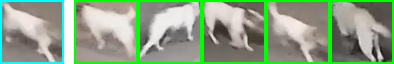
\includegraphics{images/petsearch/ranked_lists/1/collage.jpg}
	\end{subfigure}
	\par\vspace{\abovecaptionskip}
	\begin{subfigure}[b]{\textwidth}
		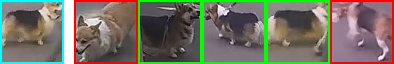
\includegraphics{images/petsearch/ranked_lists/4/collage.jpg}
	\end{subfigure}
	\par\vspace{\abovecaptionskip}
	\begin{subfigure}[b]{\textwidth}
		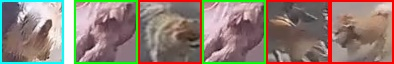
\includegraphics{images/petsearch/ranked_lists/3/collage.jpg}
	\end{subfigure}
	\par\vspace{\abovecaptionskip}
	\begin{subfigure}[b]{\textwidth}
		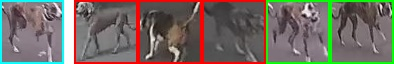
\includegraphics{images/petsearch/ranked_lists/2/collage.jpg}
	\end{subfigure}
	\caption{Пример получаемых ранжированных списков для данных камер видеонаблюдения}
	\label{fig:unicom_ranked}
\end{figure}

Можно видеть, что модель достаточно точно идентифицирует собак по общему внешнему виду, что свидетельствует о применимости подхода метрического обучения для задачи поиска собак.


\section{Анализ результатов}

Таким образом, связь задачи поиска пропавших домашних животных с задачей \reid\ состоит в применимости основных технологий, таких как метрическое обучение, оптимизация ранжирования и использование дополнительной информации.

Однако домен распознавания животных является специфичным, что препятствует прямому переносу общих подходов. Так, для данной сферы не имеется достаточно больших датасетов, имеющих разметку для задачи Re-Id. Таким образом, речь идет не о полном обучении или finetuning-е классических моделей ре-идентификации, а объединении их с дополнительной информацией, специфичной для домена поиска животных.

Так, нейросеть метрического обучения, показывающая высокое качество на некоторых бенчмарках, показывает визуально приемлемые результаты применения в поиске собак. Однако есть и ситуации, свидетельствующие о необходимости использования дополнительной информации для улучшения качества ее работы. Так, например, на \hyperref[fig:confusion]{Рисунке \ref*{fig:confusion}} продемонстрирован случай, когда модель Unicom в качестве ближайшего примера для запроса \ref{fig:confusion_big} выдает изображение \ref{fig:confusion_small}, содержащее собаку, похожую по силуэту, окрасу и типу шерсти, однако относящуюся к другой породе и имеющую другой размер. Для того, чтобы корректно обрабатывать такие ситуации, также может быть полезно внесение в модель априорных знаний о доменной области, позволяющих влиять на решения в спорных ситуациях.

\begin{figure}[ht]
	\centering
	\begin{subfigure}[b]{0.33\textwidth}
		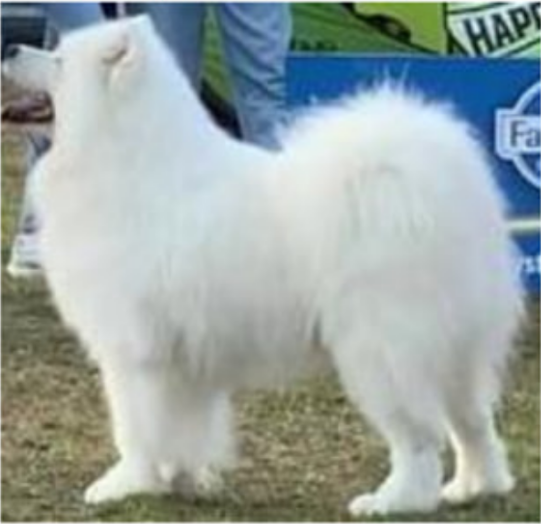
\includegraphics{images/petsearch/confusion/big.png}
		\caption{Самоед}
		\label{fig:confusion_big}
	\end{subfigure}
%	\hfill
	\begin{subfigure}[b]{0.33\textwidth}
		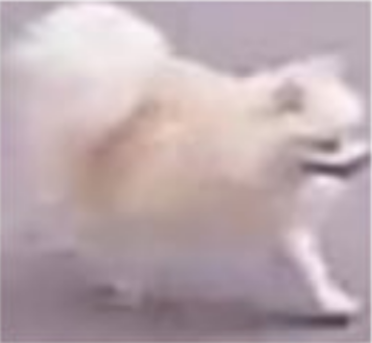
\includegraphics{images/petsearch/confusion/small.png}
		\caption{Чихуахуа}
		\label{fig:confusion_small}
	\end{subfigure}
	\caption{Пример сложного случая}
	\label{fig:confusion}
\end{figure}

Таким образом, проведенные эксперименты свидетельствуют о том, что для оптимальной работы системы поиска на основе Re-Id необходимо учитывать дополнительную информацию, специфичную для доменной области. Это приводит нас к рассмотрению state-of-the-art подхода ре-идентификации CLIP-ReID, позволяющему строить текстовые и визуальные представления.



\endinput